\documentclass[11pt,a4paper]{ctexart}
% Shared preamble for the assignment reports. Use with:
%   \documentclass[11pt,a4paper]{ctexart}  (XeLaTeX)
%   % Shared preamble for the assignment reports. Use with:
%   \documentclass[11pt,a4paper]{ctexart}  (XeLaTeX)
%   % Shared preamble for the assignment reports. Use with:
%   \documentclass[11pt,a4paper]{ctexart}  (XeLaTeX)
%   \input{../common/preamble.tex}
\usepackage[margin=2.3cm]{geometry}
\setmainfont{texgyretermes}[Extension=.otf,UprightFont=*-regular,BoldFont=*-bold,ItalicFont=*-italic,BoldItalicFont=*-bolditalic]
\setsansfont{texgyreheros}[Extension=.otf,UprightFont=*-regular,BoldFont=*-bold,ItalicFont=*-italic,BoldItalicFont=*-bolditalic]
\setmonofont{texgyrecursor}[Extension=.otf,UprightFont=*-regular,BoldFont=*-bold,ItalicFont=*-italic,BoldItalicFont=*-bolditalic]
\usepackage{amsmath,amssymb,mathtools,bm}
\usepackage{graphicx}
\usepackage{booktabs,multirow,makecell,array,tabularx}
\usepackage[table]{xcolor}
\usepackage[most]{tcolorbox}
\usepackage{enumitem}
\usepackage{listings}
\usepackage{subcaption}
\usepackage{siunitx}
\usepackage[hidelinks]{hyperref}
\usepackage[nameinlink,noabbrev]{cleveref}
\usepackage{float}

\setlength{\emergencystretch}{3em}
\linespread{1.15}
\setlist{leftmargin=*,itemsep=2pt,topsep=3pt}
\graphicspath{{figures/}}

\crefname{figure}{图}{图}
\crefname{table}{表}{表}
\crefname{section}{第}{第}
\creflabelformat{section}{#2#1#3 节}
\crefname{equation}{式}{式}
\crefformat{equation}{式~(#2#1#3)}

\lstset{basicstyle=\ttfamily\footnotesize,columns=fullflexible,breaklines=true,frame=single,
  framerule=0.3pt,rulecolor=\color{black!40},backgroundcolor=\color{black!3},
  keywordstyle=\color{blue!60!black}\bfseries,commentstyle=\color{green!40!black},
  numbers=left,numberstyle=\tiny\color{black!50},xleftmargin=1.5em}

% Interview boxes: question, model answer, common wrong answer.
\newtcolorbox{iqbox}[1]{enhanced,breakable,colback=blue!3,colframe=blue!45!black,boxrule=0.5pt,arc=1.5pt,
  left=4pt,right=4pt,top=3pt,bottom=3pt,fonttitle=\bfseries\small,title={面试追问：#1}}
\newtcolorbox{findingbox}[1][]{enhanced,breakable,colback=green!3,colframe=green!40!black,boxrule=0.5pt,arc=1.5pt,
  left=4pt,right=4pt,top=3pt,bottom=3pt,fonttitle=\bfseries\small,title={结论#1}}
\newtcolorbox{caveatbox}{enhanced,breakable,colback=orange!4,colframe=orange!60!black,boxrule=0.5pt,arc=1.5pt,
  left=4pt,right=4pt,top=3pt,bottom=3pt,fonttitle=\bfseries\small,title={不能推出的结论}}

\newcommand{\authorline}{ShaneLiu04\thanks{GitHub: \url{https://github.com/ShaneLiu04}。代码与原始指标见 edge-deploy 仓库各 lab 的 \texttt{artifacts/raw/}。本文基于公开课程材料独立完成，与课程团队无隶属关系。}}

\usepackage[margin=2.3cm]{geometry}
\setmainfont{texgyretermes}[Extension=.otf,UprightFont=*-regular,BoldFont=*-bold,ItalicFont=*-italic,BoldItalicFont=*-bolditalic]
\setsansfont{texgyreheros}[Extension=.otf,UprightFont=*-regular,BoldFont=*-bold,ItalicFont=*-italic,BoldItalicFont=*-bolditalic]
\setmonofont{texgyrecursor}[Extension=.otf,UprightFont=*-regular,BoldFont=*-bold,ItalicFont=*-italic,BoldItalicFont=*-bolditalic]
\usepackage{amsmath,amssymb,mathtools,bm}
\usepackage{graphicx}
\usepackage{booktabs,multirow,makecell,array,tabularx}
\usepackage[table]{xcolor}
\usepackage[most]{tcolorbox}
\usepackage{enumitem}
\usepackage{listings}
\usepackage{subcaption}
\usepackage{siunitx}
\usepackage[hidelinks]{hyperref}
\usepackage[nameinlink,noabbrev]{cleveref}
\usepackage{float}

\setlength{\emergencystretch}{3em}
\linespread{1.15}
\setlist{leftmargin=*,itemsep=2pt,topsep=3pt}
\graphicspath{{figures/}}

\crefname{figure}{图}{图}
\crefname{table}{表}{表}
\crefname{section}{第}{第}
\creflabelformat{section}{#2#1#3 节}
\crefname{equation}{式}{式}
\crefformat{equation}{式~(#2#1#3)}

\lstset{basicstyle=\ttfamily\footnotesize,columns=fullflexible,breaklines=true,frame=single,
  framerule=0.3pt,rulecolor=\color{black!40},backgroundcolor=\color{black!3},
  keywordstyle=\color{blue!60!black}\bfseries,commentstyle=\color{green!40!black},
  numbers=left,numberstyle=\tiny\color{black!50},xleftmargin=1.5em}

% Interview boxes: question, model answer, common wrong answer.
\newtcolorbox{iqbox}[1]{enhanced,breakable,colback=blue!3,colframe=blue!45!black,boxrule=0.5pt,arc=1.5pt,
  left=4pt,right=4pt,top=3pt,bottom=3pt,fonttitle=\bfseries\small,title={面试追问：#1}}
\newtcolorbox{findingbox}[1][]{enhanced,breakable,colback=green!3,colframe=green!40!black,boxrule=0.5pt,arc=1.5pt,
  left=4pt,right=4pt,top=3pt,bottom=3pt,fonttitle=\bfseries\small,title={结论#1}}
\newtcolorbox{caveatbox}{enhanced,breakable,colback=orange!4,colframe=orange!60!black,boxrule=0.5pt,arc=1.5pt,
  left=4pt,right=4pt,top=3pt,bottom=3pt,fonttitle=\bfseries\small,title={不能推出的结论}}

\newcommand{\authorline}{ShaneLiu04\thanks{GitHub: \url{https://github.com/ShaneLiu04}。代码与原始指标见 edge-deploy 仓库各 lab 的 \texttt{artifacts/raw/}。本文基于公开课程材料独立完成，与课程团队无隶属关系。}}

\usepackage[margin=2.3cm]{geometry}
\setmainfont{texgyretermes}[Extension=.otf,UprightFont=*-regular,BoldFont=*-bold,ItalicFont=*-italic,BoldItalicFont=*-bolditalic]
\setsansfont{texgyreheros}[Extension=.otf,UprightFont=*-regular,BoldFont=*-bold,ItalicFont=*-italic,BoldItalicFont=*-bolditalic]
\setmonofont{texgyrecursor}[Extension=.otf,UprightFont=*-regular,BoldFont=*-bold,ItalicFont=*-italic,BoldItalicFont=*-bolditalic]
\usepackage{amsmath,amssymb,mathtools,bm}
\usepackage{graphicx}
\usepackage{booktabs,multirow,makecell,array,tabularx}
\usepackage[table]{xcolor}
\usepackage[most]{tcolorbox}
\usepackage{enumitem}
\usepackage{listings}
\usepackage{subcaption}
\usepackage{siunitx}
\usepackage[hidelinks]{hyperref}
\usepackage[nameinlink,noabbrev]{cleveref}
\usepackage{float}

\setlength{\emergencystretch}{3em}
\linespread{1.15}
\setlist{leftmargin=*,itemsep=2pt,topsep=3pt}
\graphicspath{{figures/}}

\crefname{figure}{图}{图}
\crefname{table}{表}{表}
\crefname{section}{第}{第}
\creflabelformat{section}{#2#1#3 节}
\crefname{equation}{式}{式}
\crefformat{equation}{式~(#2#1#3)}

\lstset{basicstyle=\ttfamily\footnotesize,columns=fullflexible,breaklines=true,frame=single,
  framerule=0.3pt,rulecolor=\color{black!40},backgroundcolor=\color{black!3},
  keywordstyle=\color{blue!60!black}\bfseries,commentstyle=\color{green!40!black},
  numbers=left,numberstyle=\tiny\color{black!50},xleftmargin=1.5em}

% Interview boxes: question, model answer, common wrong answer.
\newtcolorbox{iqbox}[1]{enhanced,breakable,colback=blue!3,colframe=blue!45!black,boxrule=0.5pt,arc=1.5pt,
  left=4pt,right=4pt,top=3pt,bottom=3pt,fonttitle=\bfseries\small,title={面试追问：#1}}
\newtcolorbox{findingbox}[1][]{enhanced,breakable,colback=green!3,colframe=green!40!black,boxrule=0.5pt,arc=1.5pt,
  left=4pt,right=4pt,top=3pt,bottom=3pt,fonttitle=\bfseries\small,title={结论#1}}
\newtcolorbox{caveatbox}{enhanced,breakable,colback=orange!4,colframe=orange!60!black,boxrule=0.5pt,arc=1.5pt,
  left=4pt,right=4pt,top=3pt,bottom=3pt,fonttitle=\bfseries\small,title={不能推出的结论}}

\newcommand{\authorline}{ShaneLiu04\thanks{GitHub: \url{https://github.com/ShaneLiu04}。代码与原始指标见 edge-deploy 仓库各 lab 的 \texttt{artifacts/raw/}。本文基于公开课程材料独立完成，与课程团队无隶属关系。}}

\graphicspath{{../../solutions/mit6.5940/lab2-quantization/artifacts/figures/}}

\title{MIT 6.5940 Lab 2 实验报告：\\端侧 CNN 的 int8 量化——校准器失效、误差定位、混合精度与五种子置信区间}
\author{\authorline}
\date{2026 年 11 月}

\begin{document}
\maketitle

\begin{abstract}
MIT 6.5940（TinyML and Efficient Deep Learning）Lab 2 在 VGG 上做 k-means 与线性量化。本报告把它换成部署链路上真正会遇到的问题：
在 CIFAR-10 上训练一个 20.9 万参数、857 万 MAC 的 MobileNetV2 式网络（倒残差、ReLU6、线性瓶颈、残差），
依次研究 BN 折叠、权重粒度、5 种激活校准器、逐点误差定位、按敏感度的混合精度、QAT 与 ONNX Runtime 落地。
单次实验在 4 核 CPU 上完成；为了把结论放进置信区间，又在 RTX 6000D 上重训 5 个种子，并在服务器 CPU 上对每个模型重跑全部量化实验。

主要结论：
（a）TensorRT 式 KL 校准在这个网络上把 W8A8 从 88.1\% 拉到 63.57\%（5 个种子配对差 $-24.6\pm2.4$ 个点，A6 时 $-69.9$），
原因是 ReLU6 输出里的大量精确零：合并 bin 时它们被摊薄到相邻 bin，给 KL 加了一项只随截断点增大的惩罚，阈值中位数只有 MSE 阈值的 $0.267\pm0.002$ 倍；
去掉零 bin 后回到 fp32 的 0.1 个点以内；
（b）逐张量 W4 不仅均值差（$-11.8$ 对逐通道 $-2.3$ 个点），种子间标准差也大 10 倍，误差主要来自每通道只有 9 个权重的 depthwise 层；
（c）同样把 8 层升到 W8，按敏感度 $-0.63\pm0.29$、按参数量 $-2.05\pm0.54$，且少用 60 KiB；但最敏感的层随种子变化，敏感度排序必须对每个模型重测；
（d）3 个 epoch 的 QAT 把 W4A8 从 $-2.31$ 拉回 $-0.19\pm0.16$；
（e）ONNX Runtime int8 QDQ 88.09\%，单线程延迟 372.4 → 253.9 µs（1.47 倍）。
\end{abstract}

\tableofcontents
\newpage

\section{问题与模型}

端侧 CNN 量化与 VGG 量化的区别在结构：depthwise 卷积每个输出通道只有 $3\times3=9$ 个权重，通道间范围差异极大；
线性瓶颈（project 1×1 之后没有激活）让误差直接进入残差流；ReLU6 让激活分布在 0 处有一个质量很大的点。
本实验的网络（\texttt{code/edgequant/model.py}）就是为了覆盖这三个结构：stem 3×3 → 倒残差块（1×1 expand、3×3 depthwise、1×1 project、残差）× 若干 → 1×1 head → 全局池化 → FC。
26 个权重层、31 个激活量化点（与整数图里的 requant 位置一一对应，\texttt{test\_points\_follow\_execution\_order}）。

\begin{table}[H]
\centering\small
\caption{实验链路}\label{tab:pipeline}
\begin{tabularx}{\linewidth}{l >{\raggedright\arraybackslash}X}
\toprule
步骤 & 内容 \\
\midrule
BN 折叠 & $W' = \gamma W/\sigma$，$b' = \gamma(b-\mu)/\sigma + \beta$；fp32 88.16\% → 88.16\%，logits 最大差 $4.9\times10^{-6}$ \\
权重粒度 & 逐张量 / 逐通道 / 逐通道但 depthwise 逐张量，W8/W6/W4 \\
激活校准 & minmax、percentile 99.99、MSE、KL（TensorRT 式 2048 bin → 128 级）、KL 去零 bin；512 张校准图 \\
误差定位 & 一次只量化一个点；沿深度的逐点 SQNR；逐层单独 W4 的敏感度 \\
混合精度 & W4 起步，按敏感度或按参数量逐层升到 W8 \\
QAT & W4A8，直通估计（STE）只在裁剪区间内传梯度，3 个 epoch \\
部署 & ONNX QDQ → ORT 图融合成 QLinearConv，1 线程延迟 \\
\bottomrule
\end{tabularx}
\end{table}

\section{权重粒度}

\begin{table}[H]
\centering\small
\caption{只量化权重的精度（\%，单次训练 seed 0）}\label{tab:gran}
\begin{tabular}{lrrr}
\toprule
位宽 & 逐通道 & 逐张量 & 逐通道，但 depthwise 逐张量 \\
\midrule
W8 & 88.16 & 88.15 & 88.13 \\
W6 & 88.02 & 87.20 & 87.68 \\
W4 & 83.20 & 76.42 & 82.06 \\
\bottomrule
\end{tabular}
\end{table}

\begin{figure}[H]
\centering
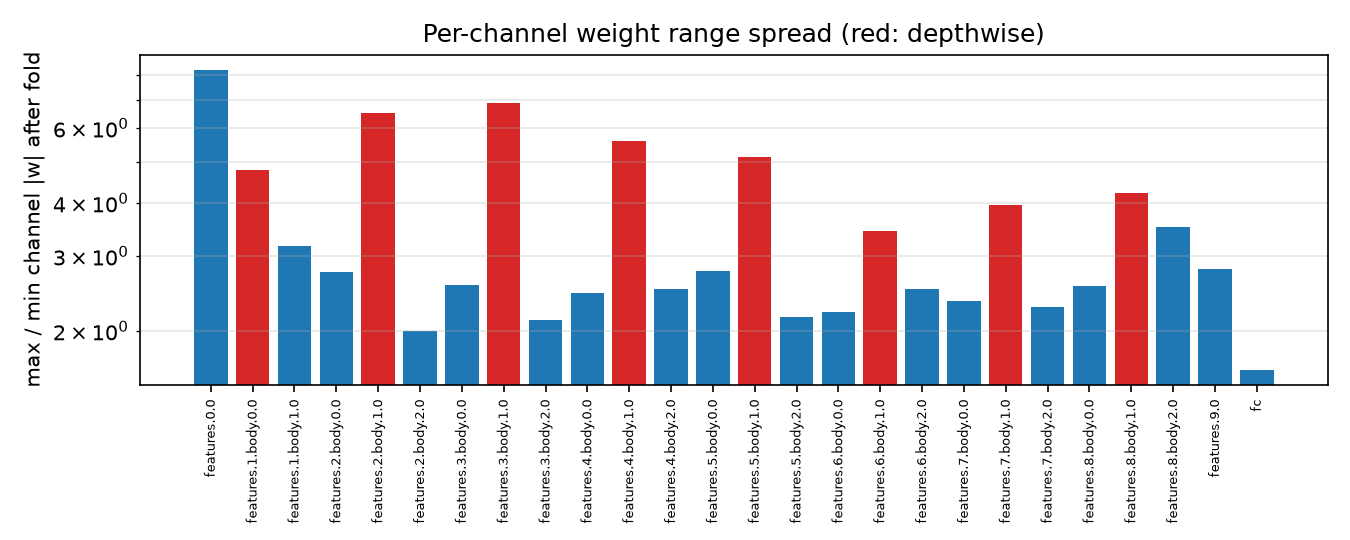
\includegraphics[width=0.9\linewidth]{weight_ranges.png}
\caption{每层各输出通道 $|w|_{\max}$ 的极差（最大通道 / 最小通道）与逐张量 W8 下最差通道的相对误差。}\label{fig:ranges}
\end{figure}

逐张量量化的步长由全层最大的通道决定：$\Delta = \max_c |w_c|_{\max} / (2^{b-1}-1)$。一个 $|w|_{\max}$ 只有最大通道 1/10 的通道，
在 W4 下只剩不到 1 个量化级，整个通道被量化成 0。depthwise 层每通道 9 个权重、没有跨通道求和来平均误差，所以“只把 depthwise 改回逐张量”就损失 1.1 个点（W4）。
误差按位宽放大：W8 时三种粒度几乎相同，W4 时差 6.8 个点——量化噪声功率 $\propto \Delta^2 \propto 4^{-b}$，每少 1 bit 噪声大 4 倍（6 dB）。

\section{激活校准：KL 为什么崩溃}\label{sec:kl}

\begin{table}[H]
\centering\small
\caption{激活校准器（权重 W8 逐通道，\%，seed 0）}\label{tab:calib}
\begin{tabular}{lrrr}
\toprule
校准器 & A8 & A6 & 耗时 \\
\midrule
minmax & 87.97 & 87.62 & 7 s \\
percentile 99.99 & 88.17 & 88.00 & 7 s \\
MSE & 88.13 & 87.94 & 25 s \\
KL（TensorRT 式） & \textbf{63.68} & \textbf{16.30} & 15 s \\
KL（去掉精确零） & 88.06 & 87.97 & 15 s \\
\bottomrule
\end{tabular}
\end{table}

\subsection{机制}
TensorRT 式 KL 校准把激活直方图分成 2048 个 bin，对每个候选截断点 $i$（$i \ge 128$），把前 $i$ 个 bin 合并成 128 组得到量化后的分布 $Q$，
与截断（尾部质量折叠进最后一个 bin）后的原分布 $P$ 比较，取 $\mathrm{KL}(P\|Q)$ 最小的 $i$。合并时，每组的质量平均分给组内\emph{非零}的 bin。

ReLU6 之后，相当比例的激活恰好是 0，全部落在第 0 个 bin，质量为 $p_0$。第 0 组包含 $i/128$ 个 bin，合并后 $Q$ 把 $p_0$ 摊给组内所有非零 bin，
于是第 0 个 bin 上 $Q_0 \approx p_0 \cdot 128/i$（若组内其他 bin 也非零）。这一项对 KL 的贡献约为
\[
  p_0 \ln \frac{P_0}{Q_0} \approx p_0 \ln \frac{i}{128},
\]
\emph{只随截断点 $i$ 增大}，与真实的量化误差无关——在真实的整数执行里，零点精确表示 0，这些激活的误差是 0。
$p_0$ 越大，这一项越压过尾部的裁剪误差，搜索就越偏向小阈值。实测 ReLU 后的激活点上 KL 阈值中位数只有 MSE 最优阈值的 0.268 倍，
大量正常激活被裁剪。把第 0 个 bin 从直方图中拿掉再做同样的搜索（“KL 去零”），比值回到 0.733，精度回到 88.06\%。

\begin{figure}[H]
\centering
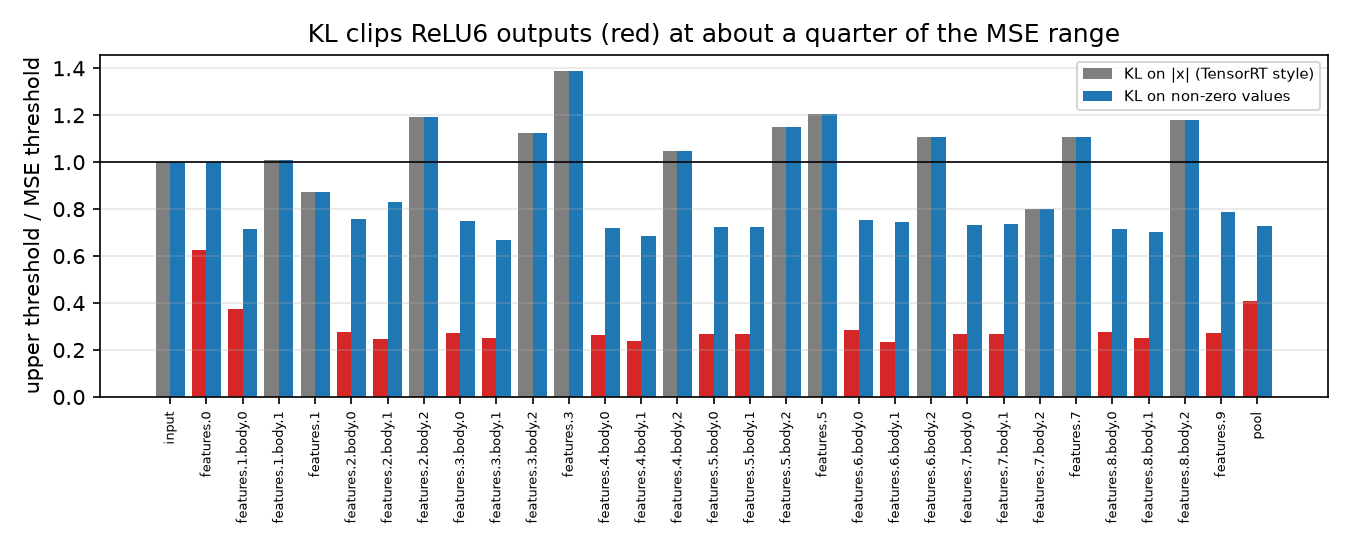
\includegraphics[width=0.9\linewidth]{kl_points.png}
\caption{每个激活点 KL 阈值 / MSE 阈值（去零前后），以及只把这一个点换成 KL 阈值时的精度损失。}\label{fig:kl}
\end{figure}

单独把一个点换成 KL 阈值，最坏只掉 6.96 个点；31 个点一起换掉 24 个点——误差沿深度累积，单点定位找不到“罪魁祸首层”，只能找到“罪魁祸首分布”。
校准集大小不是原因：从 8 张增到 2048 张，A6 精度波动不到 0.12 个点（各 3 次重复）。

\begin{iqbox}{TensorRT 默认用 entropy（KL）校准，为什么在你的模型上不行？}
KL 校准隐含假设“直方图每个 bin 的质量都需要被量化网格表示”。ReLU / ReLU6 之后有大量精确零，它们在整数执行中被零点精确表示、没有误差，
但 KL 在合并 bin 时把这块质量摊到相邻 bin，产生一项只随截断点增大的伪惩罚，于是阈值被压到 MSE 最优值的约 1/4。
修法：从直方图中去掉零 bin，或者对 ReLU 后的点改用 MSE / percentile。验收时不能只看校准器名字，要看每个点的阈值比。
ORT 的 Entropy 校准默认参数下不掉点，但那是因为它根本没做搜索（\cref{sec:ortseeds}）；改成 2048 bin 才真的搜索，掉到 87.17\%。
\end{iqbox}

\section{误差定位与混合精度}

\begin{figure}[H]
\centering
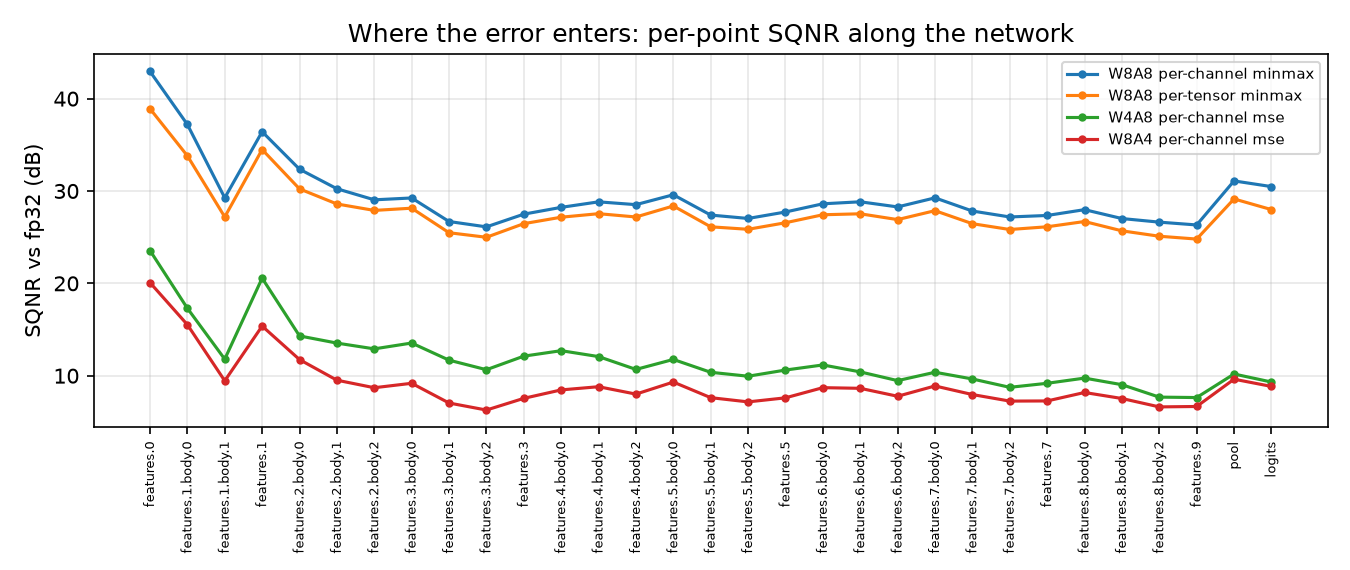
\includegraphics[width=0.9\linewidth]{localize.png}
\caption{沿深度的逐激活点 SQNR。}\label{fig:localize}
\end{figure}

逐点 SQNR（\cref{fig:localize}）：W8A8 在 26.1--42.9 dB；W4A8 时 depthwise 输出 17.3 dB、project 输出 11.8 dB、残差相加后 20.6 dB。
误差在线性瓶颈处进入：project 层没有 ReLU 截掉负的误差，而残差相加把较干净的捷径信号加回来，SQNR 回升。
逐层单独 W4，最敏感的是 \texttt{features.2.body.2.0}（掉 0.71 个点）；26 层单独掉点之和 4.23，全部同时 W4 掉 4.96——\emph{敏感度不可加}，层间误差会相互放大。

\begin{figure}[H]
\centering
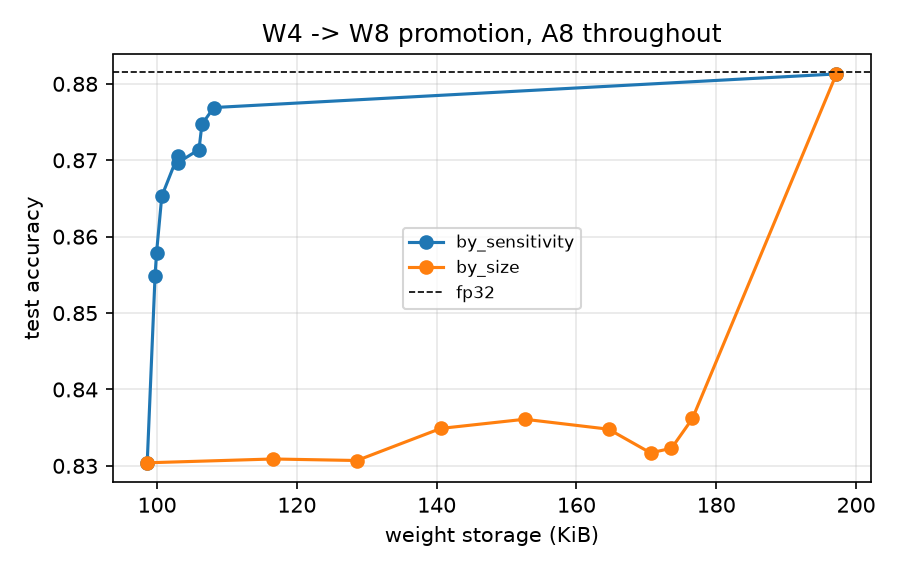
\includegraphics[width=0.75\linewidth]{mixed_precision.png}
\caption{从全 W4 出发逐层升到 W8：按敏感度 vs 按参数量（seed 0）。}\label{fig:mixed}
\end{figure}

\begin{table}[H]
\centering\small
\caption{混合精度（seed 0）}\label{tab:mixed}
\begin{tabular}{rll}
\toprule
升到 W8 的层数 & 按敏感度 & 按参数量 \\
\midrule
0 & 83.04\%，98.6 KiB & 83.04\%，98.6 KiB \\
4 & 87.05\%，102.9 KiB & 83.61\%，152.6 KiB \\
8 & 87.69\%，108.1 KiB & 83.62\%，176.6 KiB \\
26（全 W8） & 88.13\%，197.2 KiB & 88.13\%，197.2 KiB \\
\bottomrule
\end{tabular}
\end{table}

最大的几层是网络后部的 pointwise，参数多但不敏感（输入通道多，误差在求和中平均掉）；敏感层是前面的小层。按参数量升 8 层花了 78 KiB 只回来 0.6 个点，
按敏感度升 8 层只花 9.5 KiB 回来 4.65 个点。

\section{QAT 与部署}

W4A8 QAT 从 PTQ 的 83.04\% 起步，三个 epoch 后 87.49 → 87.50 → 87.63\%，每个 epoch 约 110 s。STE 只在裁剪区间内传梯度：
$\partial \hat{x}/\partial x = \mathbb{1}[q_{\min}\le x/s \le q_{\max}]$，区间外梯度为 0，否则被裁剪的权重会被推得更远。

\begin{table}[H]
\centering\small
\caption{ONNX Runtime 1.31 部署（batch 1，1 线程）}\label{tab:ort}
\begin{tabular}{lrrr}
\toprule
模型 & 精度 \% & 延迟 µs & 文件 KiB \\
\midrule
fp32 折叠 & 88.16 & 372.4 & 823.7 \\
int8 QDQ MinMax & 88.09 & 253.9 & 318.5 \\
int8 QDQ Entropy（默认） & 88.09 & 270.7 & 318.5 \\
int8 QDQ Entropy 2048 bin & 87.17 & 262.3 & 318.5 \\
int8 QDQ Percentile & 88.06 & 264.0 & 318.5 \\
\bottomrule
\end{tabular}
\end{table}

int8 只快 1.47 倍而不是 4 倍：这个网络很小（857 万 MAC），单次推理 254 µs 里有相当部分是逐算子的调度与 requant；
depthwise 层在 ORT 4 线程下 int8 甚至比 fp32 慢（见 int8-kernels lab）。ORT 的 QLinearConv requant 语义（浮点乘、四舍六入五成双）在 int8-kernels lab 里与自写 C++ 逐位对齐过。

\section{五个种子：哪些结论经得起重训}\label{sec:seeds}

\subsection{设计}
单次训练的结论有两个噪声来源：评测噪声（1 万张图，88\% 附近标准误约 0.3 个点）与训练随机性（初始化、数据顺序）。
在 RTX 6000D 上用同样的超参数训练 5 个种子（每个 156 s，fp32 88.32 / 88.28 / 88.16 / 87.99 / 87.91\%，均值 $88.12\pm0.18$），
再在服务器 CPU 上把每个模型的全部量化实验并行重跑一遍（每个种子 4 个物理核）。

统计量用\emph{配对差} $d_s = \mathrm{acc}_s(\text{方法}) - \mathrm{acc}_s(\text{fp32})$。同一种子的 fp32 波动在差值里抵消，
所以比种子间 0.2 个点的 fp32 波动更小的方法差异也能分辨。95\% 置信区间 $\bar d \pm t_{0.975,4}\, s_d/\sqrt{5}$，$t_{0.975,4}=2.776$。

\begin{table}[H]
\centering\small
\caption{五种子配对差（个百分点）}\label{tab:seeds}
\begin{tabular}{lrrr}
\toprule
方法 & 精度均值 \% & 配对差 & 95\% CI \\
\midrule
W8A8 minmax & 88.16 & $+0.03$ & $\pm0.06$ \\
W8A8 MSE & 88.13 & $+0.01$ & $\pm0.08$ \\
\textbf{W8A8 KL} & \textbf{63.57} & $\mathbf{-24.55}$ & $\pm2.42$ \\
W8A8 KL 去零 & 88.07 & $-0.05$ & $\pm0.08$ \\
W8A6 KL & 18.26 & $-69.86$ & $\pm14.6$ \\
W8A6 KL 去零 & 87.88 & $-0.25$ & $\pm0.22$ \\
W4 逐张量 & 76.36 & $-11.76$ & $\pm4.26$ \\
W4 逐通道 & 85.86 & $-2.26$ & $\pm0.26$ \\
W4 逐通道但 depthwise 逐张量 & 82.46 & $-5.66$ & $\pm3.41$ \\
混合精度，按敏感度升 8 层 & 87.50 & $-0.63$ & $\pm0.29$ \\
混合精度，按参数量升 8 层 & 86.07 & $-2.05$ & $\pm0.54$ \\
QAT W4A8 前 / 后 & 85.81 / 87.94 & $-2.31$ / $-0.19$ & $\pm0.24$ / $\pm0.16$ \\
\bottomrule
\end{tabular}
\end{table}

\begin{figure}[H]
\centering
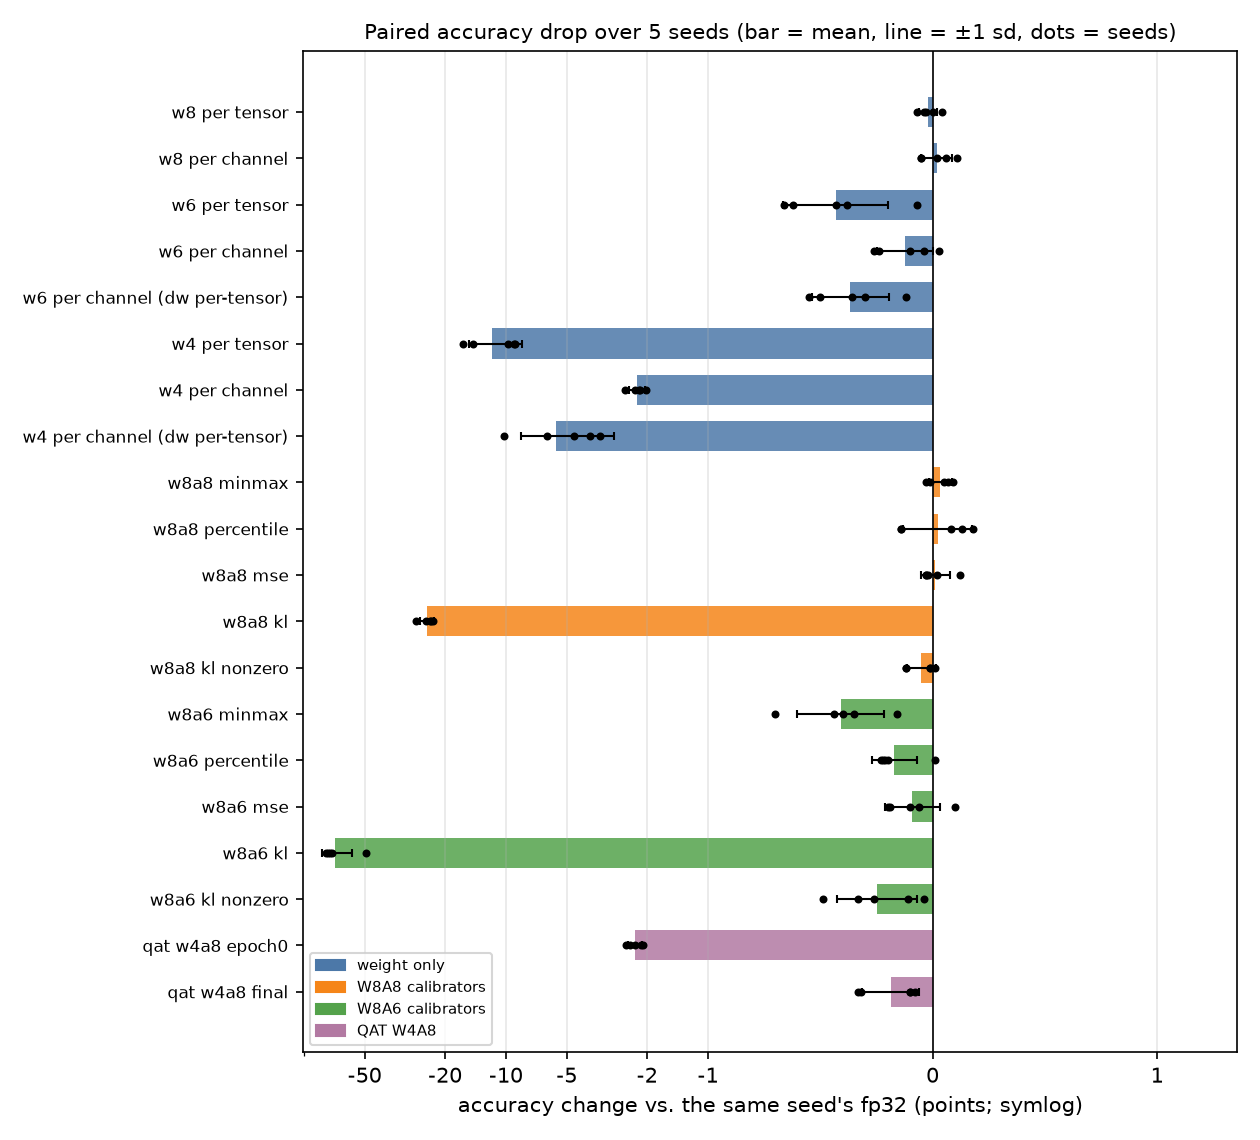
\includegraphics[width=0.82\linewidth]{seeds_quant.png}
\caption{五种子配对差（symlog 横轴；条 = 均值，误差线 = ±1 sd，点 = 各种子）。}\label{fig:seedsq}
\end{figure}

\begin{findingbox}[：结构性的结论]
KL 崩溃在 5 个种子上全部复现（60.4--65.3\%），KL/MSE 阈值比 $0.267\pm0.002$ 几乎不随种子变化——它由 ReLU6 后的零质量决定，而零质量是网络结构的性质。
混合精度“按敏感度优于按大小”的区间不重叠；QAT 的收益可复现。
\end{findingbox}

\begin{findingbox}[：随训练变化的结论]
（1）逐张量 W4 的标准差是逐通道的 10 倍（3.3 对 0.32 个点）：逐张量的步长取决于“这次训练哪个通道最大”。粒度不仅影响均值，也影响可复现性。
（2）最敏感的 W4 层并不固定：5 个种子里分别是 stem（2 次）、第一个 depthwise（1 次）、第二个块的 depthwise（2 次）。
单次实验报告的 \texttt{features.2.body.2.0} 只是 CPU 训练那一个模型的结果。
\end{findingbox}

\begin{figure}[H]
\centering
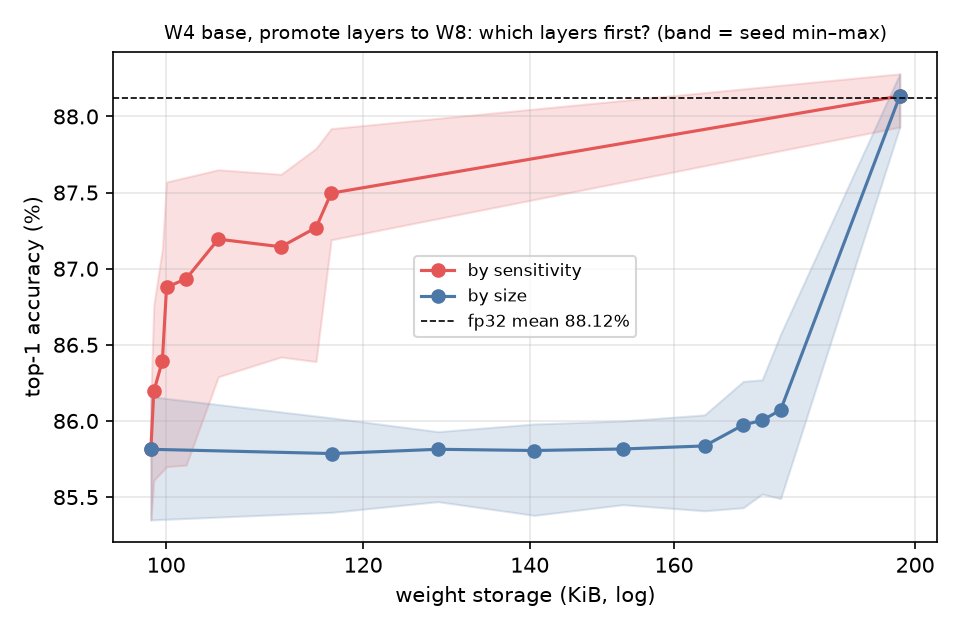
\includegraphics[width=0.7\linewidth]{seeds_mixed.png}
\caption{五种子混合精度曲线（线 = 均值，带 = 种子最小--最大）。按敏感度的曲线在存储轴上的位置各种子不同，因为选中的层不同。}\label{fig:seedsm}
\end{figure}

\begin{iqbox}{你说按敏感度做混合精度更好，那敏感度排序能复用到同结构的另一个模型上吗？}
不能直接复用。五个同结构、同超参数、只换随机种子的模型里，最敏感的层有三种不同答案。“哪类层敏感”（前部小层、depthwise）是稳定的，
“具体哪一层最敏感”不是。工程上要把逐层敏感度扫描作为每次重训后的量化流水线的一步（26 层单独 W4，约 6 分钟 CPU），
而不是把上一个模型的配置抄过来。
\end{iqbox}

\subsection{ORT 部署的五种子复现}\label{sec:ortseeds}

\begin{table}[H]
\centering\small
\caption{ORT int8 QDQ 五种子配对差（个百分点；每个种子绑 4 核、ORT 1 线程）}\label{tab:ortseeds}
\begin{tabular}{lrr}
\toprule
校准器 & 配对差 & 95\% CI \\
\midrule
MinMax & $+0.01$ & $\pm0.07$ \\
Entropy（默认参数） & $+0.01$ & $\pm0.07$ \\
Entropy，2048 bin & $-0.82$ & $\pm0.10$ \\
Percentile & $+0.04$ & $\pm0.06$ \\
\bottomrule
\end{tabular}
\end{table}

\begin{findingbox}[：ORT 的默认 Entropy 就是 MinMax]
5 个种子里 Entropy（默认）与 MinMax 的精度逐位相同。原因在 ORT 的 \texttt{calibrate.py}：
\texttt{EntropyCalibrater} 默认直方图 bin 数与量化 bin 数都是 128，阈值搜索从“量化 bin 数的一半”循环到“直方图 bin 数的一半”，
两者相等时只有一个候选，即全范围。“我们用了 KL 校准、没掉点”在默认参数下什么也没验证。
\end{findingbox}

调到 2048 bin 才是 TensorRT 式的搜索，五个种子都掉 0.7--0.9 个点，但远小于本仓库实现的 24.6。差别在直方图的坐标系：
ORT 的直方图覆盖 $[-\max|x|,\ \max|x|]$，零在正中间的 bin，候选区间以它为中心对称扩展，ReLU6 的零峰永远在切片内部；
本仓库（和 TensorRT 原始描述）的直方图是 $[0,\max]$，零峰是第一个 bin，合并时那一项 $p_0\ln(i/128)$ 随截断点单调增大（\cref{sec:kl}）。
剩下的 0.82 个点来自哪几层没有逐层定位。

服务器上 int8 的单次延迟在 120 µs 与 175 µs 两档之间跳，fp32 稳定在 201--204 µs：5 个种子同时在跑，cgroup 的 22 核配额被挤满。
快的一档相对 fp32 是 1.65 倍，与本机安静环境的 1.47 倍同量级；延迟结论以\cref{tab:ort}为准。

\begin{iqbox}{同样叫“entropy 校准”，为什么 ORT 掉 0.8 个点、你的实现掉 24 个点？}
两个原因叠加。第一，ORT 默认参数根本不搜索，等于 MinMax；要设 \texttt{num\_bins=2048} 才可比。第二，直方图坐标系不同：
ORT 以 0 为中心对称建直方图，ReLU 后的零峰在中间、永远不会被截断或与边界 bin 合并；$[0,\max]$ 的直方图里零峰是第一个 bin，
KL 合并时会产生随截断点增大的伪惩罚，把阈值压到 MSE 最优值的 1/4。所以“换一个框架同名校准器结果不同”是正常的，验收要看每个点的阈值。
\end{iqbox}

\begin{iqbox}{五个种子够吗？}
对“KL 掉 24 个点”这种效应，一个种子就够；对“按敏感度比按大小好 1.4 个点”，5 个种子的配对差给出不重叠的 95\% 区间，也够；
但对 0.05 个点量级的差异（minmax 对 MSE），区间 $\pm0.06$--$0.08$ 包含 0，不能下结论。配对设计是关键：不配对时 fp32 本身的 $\pm0.18$ 会把这些差异淹没。
\end{iqbox}

\begin{caveatbox}
\begin{itemize}
  \item 只有一个网络结构、一个数据集；KL 的失败依赖“ReLU 后大量精确零”，没有这个特征的网络里 KL 可能正常。
  \item GPU 训练的 5 个模型与 CPU 训练的 seed 0 不是同一个模型（cuDNN 的非确定性、不同的线程数），所以单次表格与五种子表格的数字不能逐项相减。
  \item ORT 延迟是本机 x86 + VNNI 单线程的数，不代表 ARM 或 MCU 上的 int8 加速比；五种子部分的 ORT 延迟是在并行负载下测的，只看精度。
  \item 敏感度扫描一次只量化一层，层间交互（不可加性）没有建模；混合精度的贪心顺序不保证最优。
\end{itemize}
\end{caveatbox}

\section{复现}

\begin{lstlisting}[language=bash,numbers=none]
cd solutions/mit6.5940/lab2-quantization
python -m pytest -q tests
python scripts/train.py                     # CPU, 4 threads, about 43 minutes
python scripts/run_experiments.py           # all 11 steps, about 30 minutes
# five seeds (GPU training, CPU evaluation)
python scripts/train.py --device cuda --seed 3 --ckpt checkpoints/seeds/micronet_s3.pt \
    --log artifacts/raw/seeds/train_log_s3.jsonl
python scripts/run_experiments.py --threads 4 --ckpt checkpoints/seeds/micronet_s3.pt \
    --out artifacts/seeds/s3 --only baseline ranges weight_only calib kl_points calib_size sensitivity localize mixed qat
python scripts/run_experiments.py --threads 1 --ckpt checkpoints/seeds/micronet_s3.pt --out artifacts/seeds/s3 --only ort
python scripts/seed_summary.py
\end{lstlisting}

\end{document}
